\chapter{Audio compressive sensing}
\label{chap:nd-cs}
In this chapter, I apply CS to audio signals. These type of signals act as the bridge to $N$-dimensional CS as they are one-dimensional when represented in the time domain, but are projected to higher dimensions when represented in another domain, such as the spectrogram/modulation domain. Unlike images, audio signals are a tad harder to compressively sample. Due to their relatively higher information density, the effects of undersampling are easily observed.

\section{Test case: Sinusoid redux}
In this test case, I recorded a guitar playing a single E$_4$ (330 Hz) note at the standard 44.1 kHz sampling rate for 4 seconds. Since the Nyquist rate of the actual signal is 660 Hz, the recording can be downsampled to a practical 8 kHz for processing. The signal waveform and frequency content is shown in Fig.~\ref{fig:guitar-original}. The base frequency is dominant in the frequency spectrum, and several harmonics can be observed. The goal here is to be able to recover the harmonics that have a frequency higher than the compressive sampling rate. The compressed signal is shown in Fig.~\ref{fig:guitar-compressed}, which was compressively sampled with a quasi-frequency of 500~Hz (500 i.i.d.~random samples per second). The waveform envelope still resembles that of the original, but due to the random nature of sampling, the periodicity is not preserved, and is reflected in the seemingly random frequency content.

\begin{figure}[htb]
	\centering
	\begin{subfigure}{\textwidth}
		\centering
		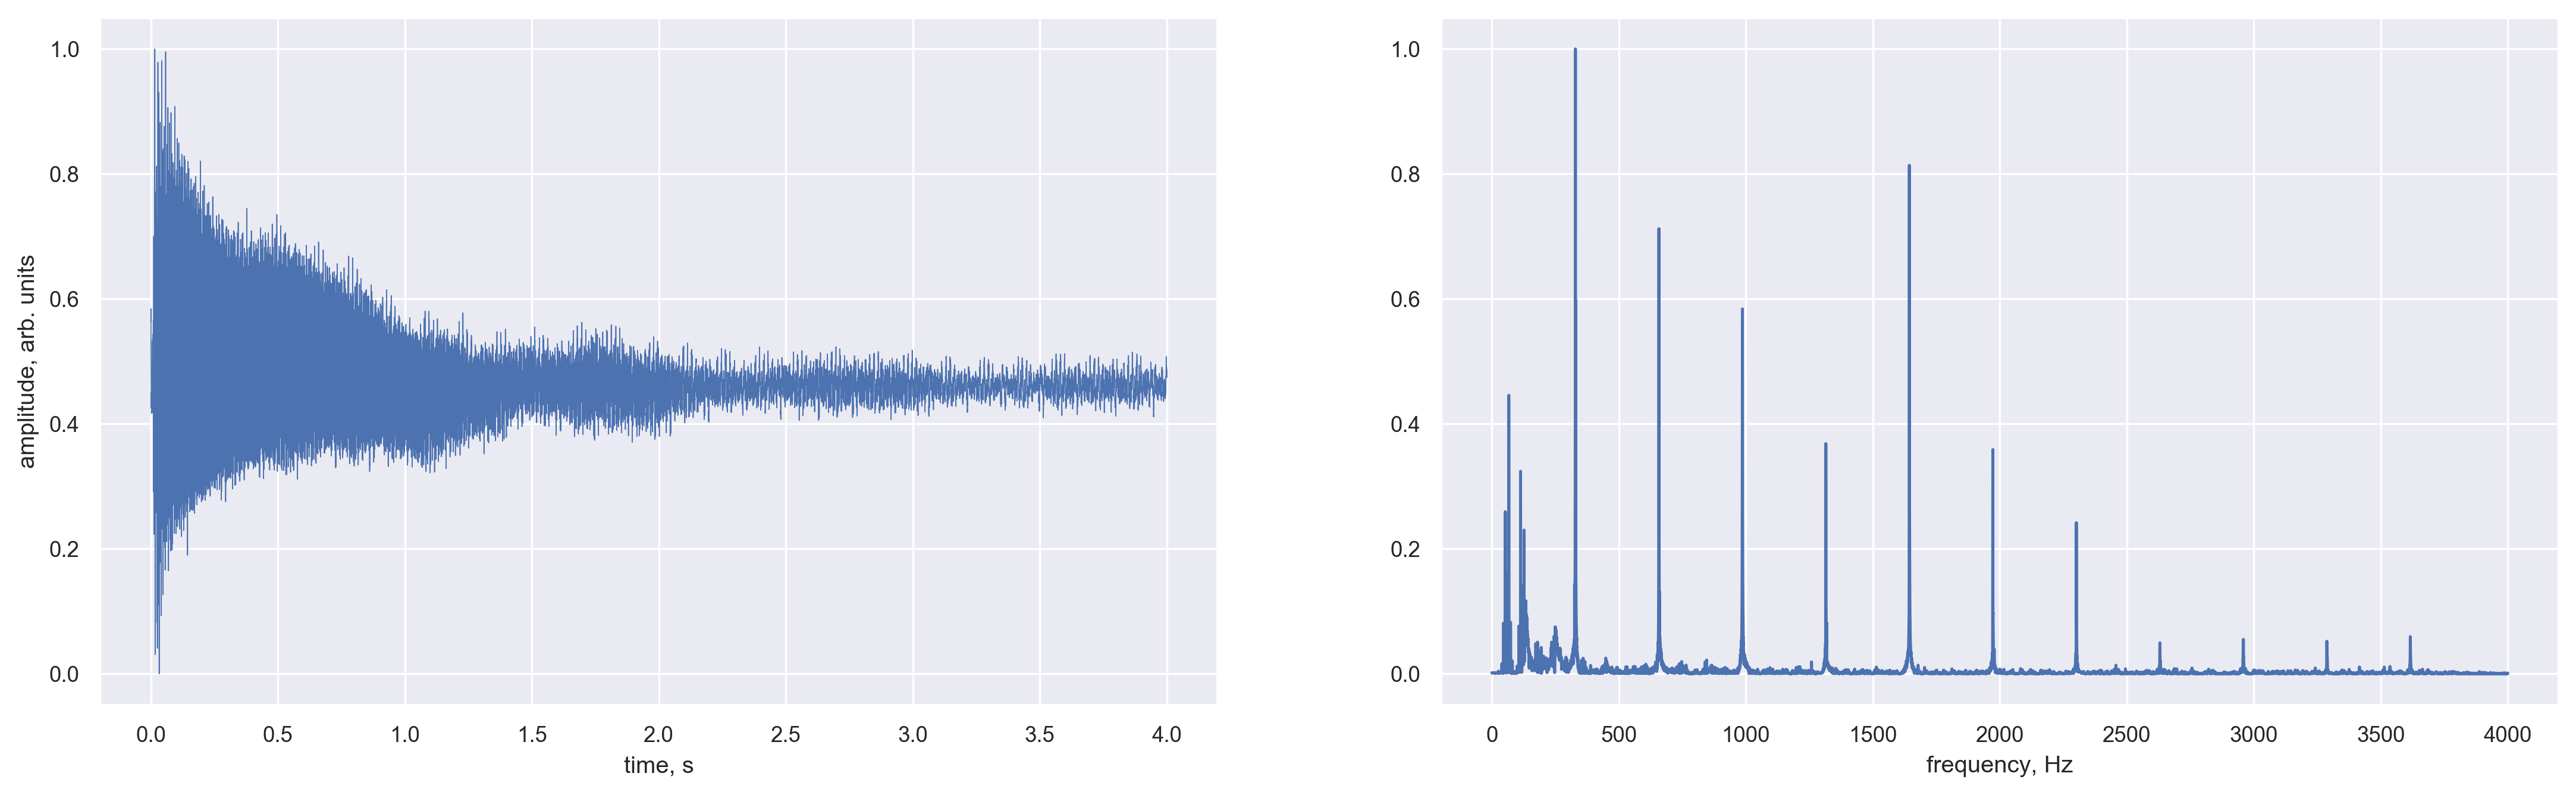
\includegraphics[width=\textwidth]{E1_orig.png}
		\caption{Original}
		\label{fig:guitar-original}
	\end{subfigure}
	\begin{subfigure}{\textwidth}
		\centering
		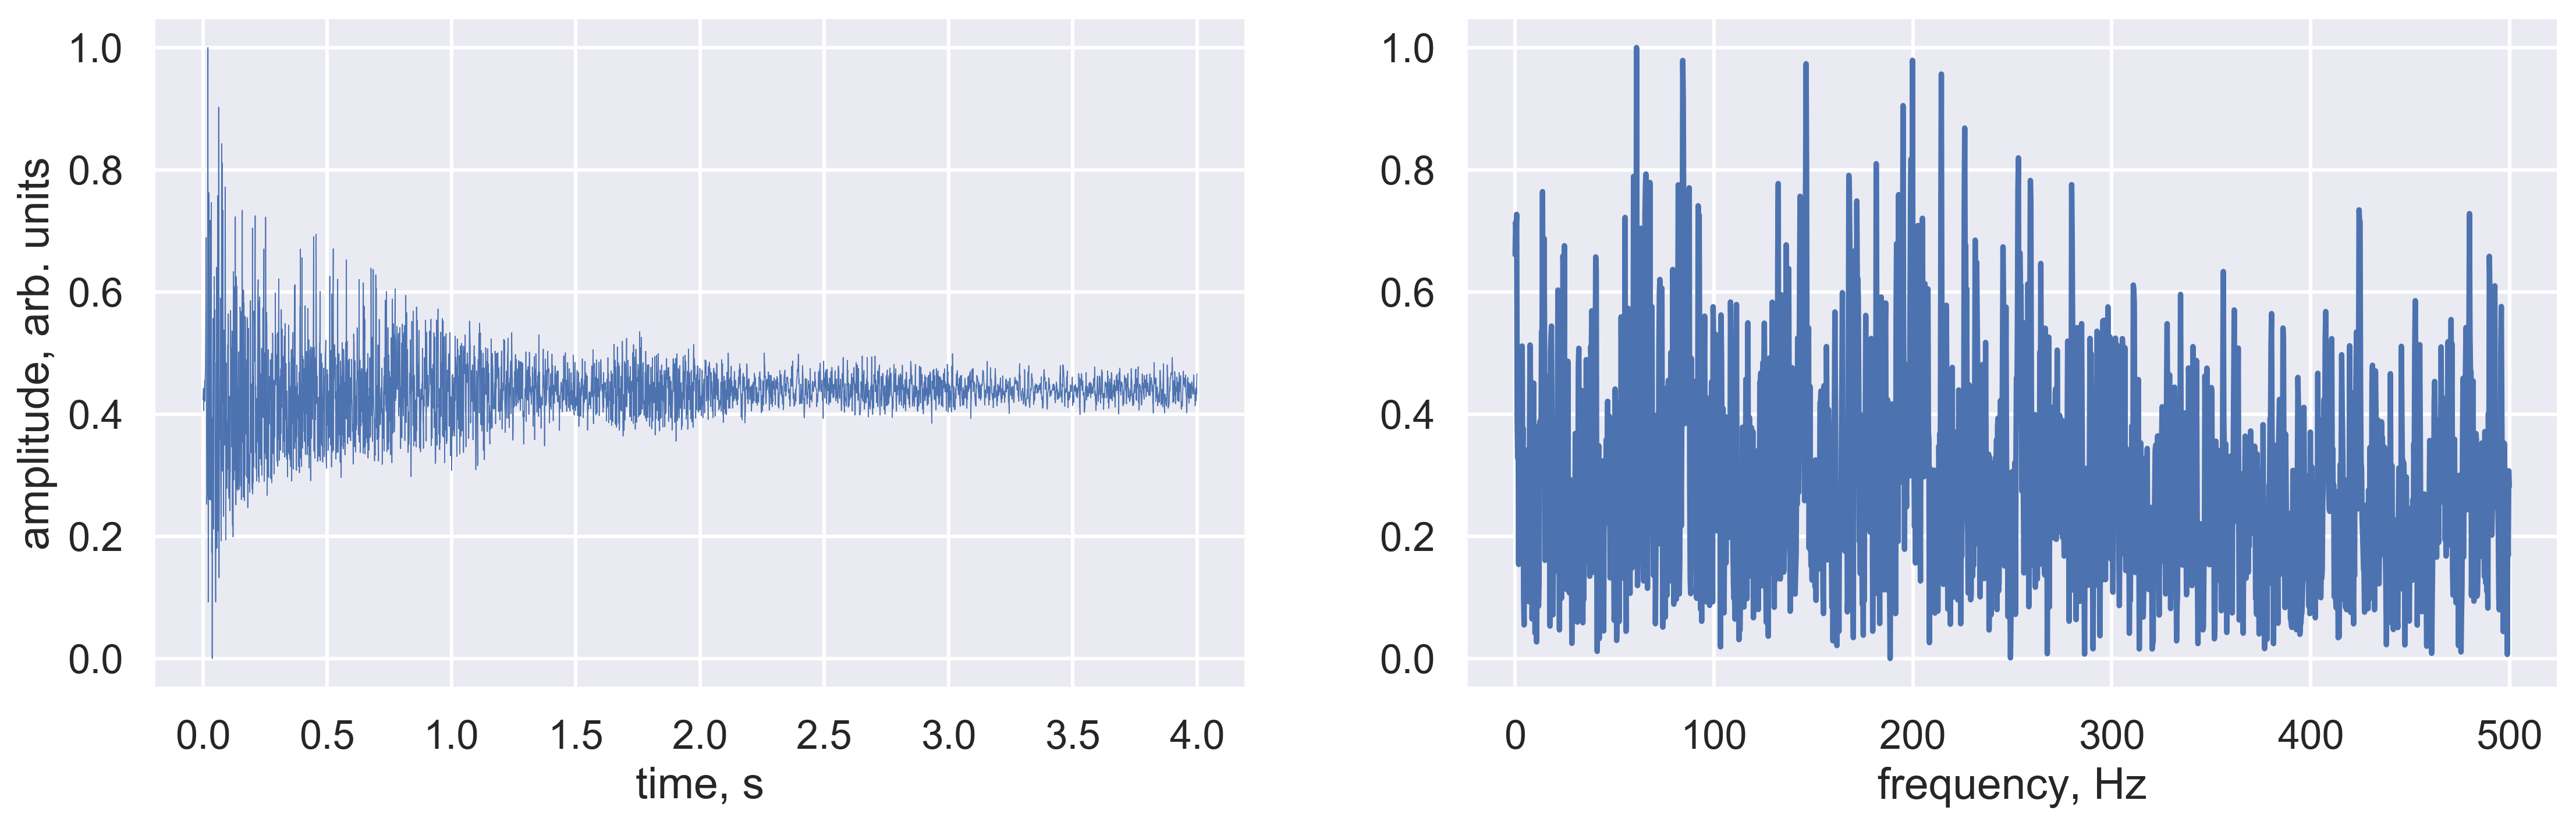
\includegraphics[width=\textwidth]{E1_comp.png}
		\caption{Compressed}
		\label{fig:guitar-compressed}
	\end{subfigure}
	\begin{subfigure}{\textwidth}
		\centering
		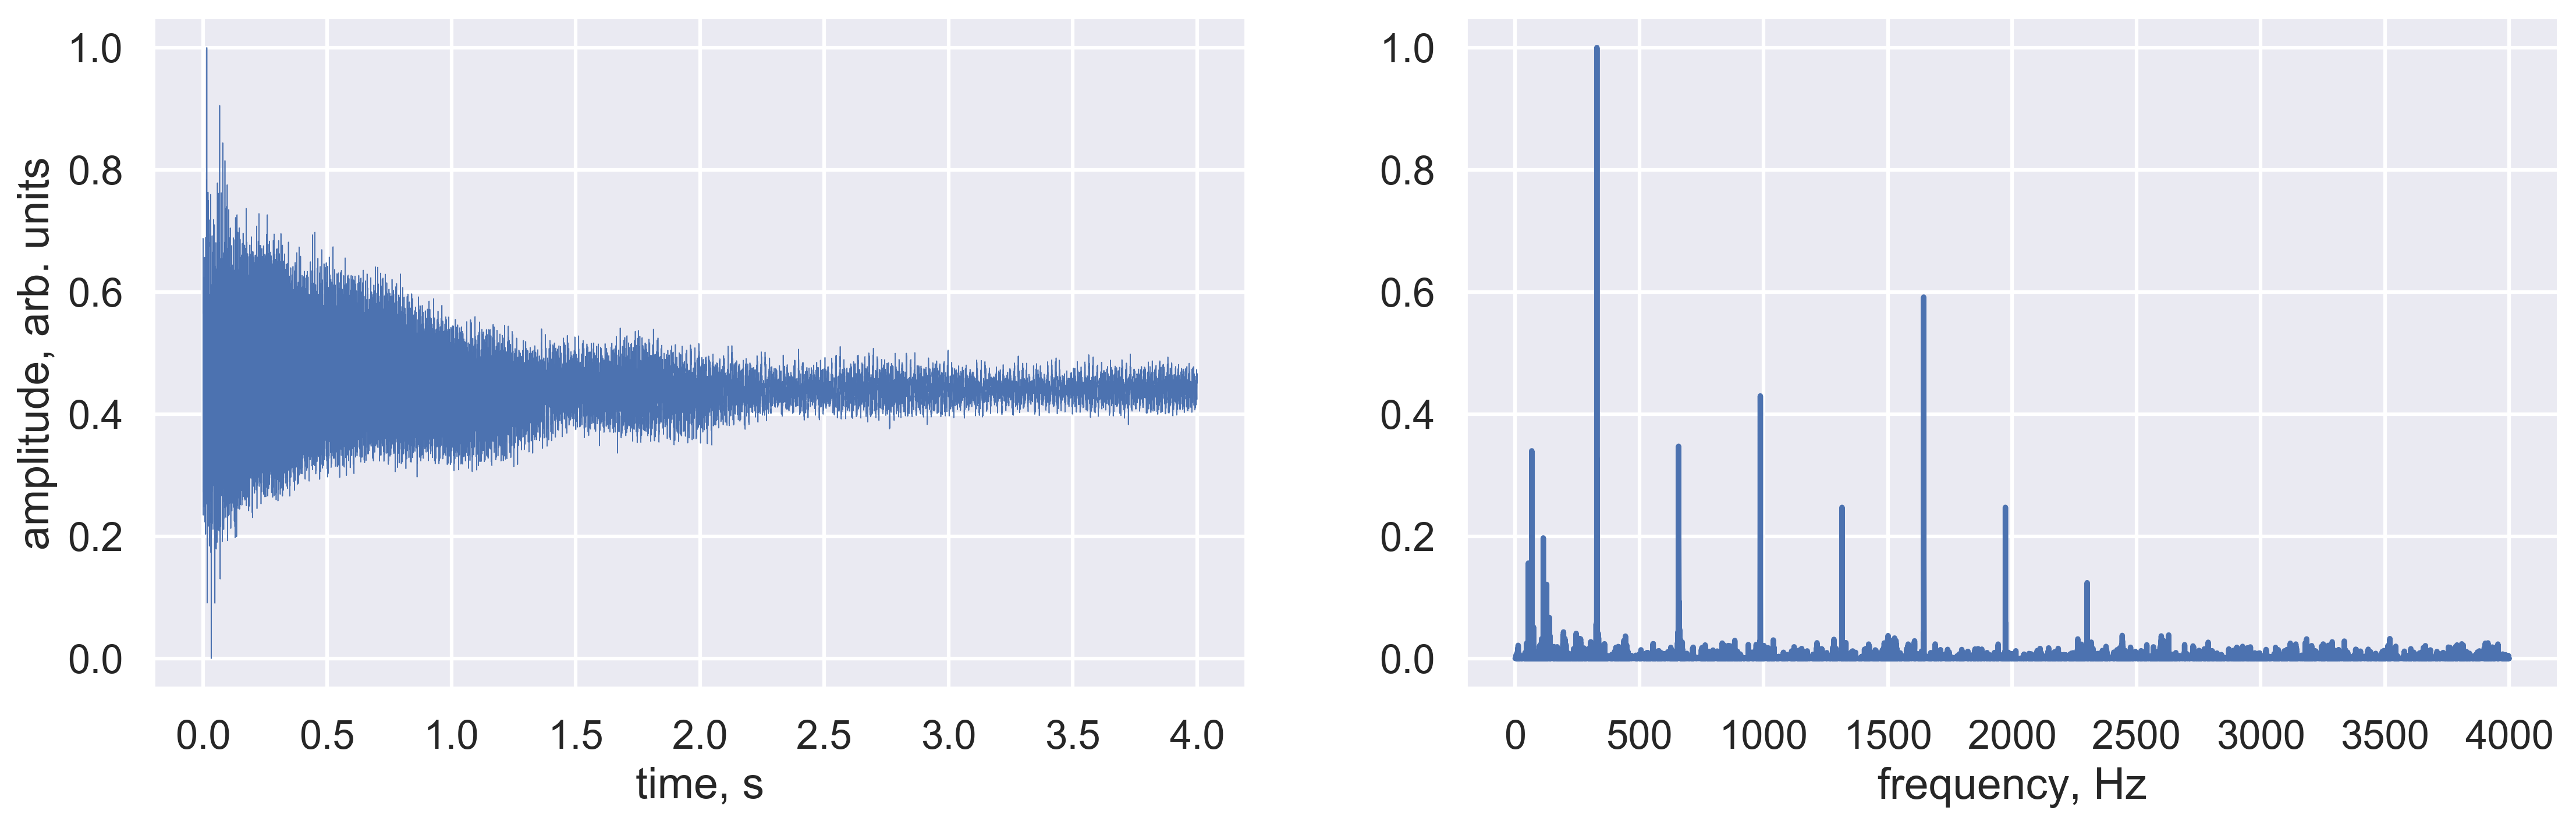
\includegraphics[width=\textwidth]{E1_recov.png}
		\caption{Recovered}
		\label{fig:guitar-recovered}
	\end{subfigure}
	\caption{330 Hz guitar signal representation in the time domain (left column) and frequency domain (right column).}
	\label{fig:guitar}
\end{figure}